% This must be in the first 5 lines to tell arXiv to use pdfLaTeX.
\pdfoutput=1

\documentclass[11pt]{article}

\usepackage[preprint]{acl}

\usepackage{times}
\usepackage{latexsym}
\usepackage[T1]{fontenc}
\usepackage[T5]{fontenc}
\usepackage[utf8]{inputenc}
\usepackage{microtype}
\usepackage{inconsolata}
\usepackage{graphicx}
\usepackage{booktabs}
\usepackage{multirow}
\usepackage{amsmath}
\usepackage{algorithm}
\usepackage{algpseudocode}
\usepackage{authblk}

\title{\textsc{SHESum}: Structure-aware Hierarchical Efficient Summarization for Vietnamese Long and Multi-Document Texts}

\author[1]{Nhat-Quang Pham}
\author[2]{Xuan-Dung Doan}
\affil[1]{University of Engineering and Technology - VNU, Vietnam \\ \texttt{pnquang05@gmail.com}}
\affil[2]{Viettel Artificial Intelligence Center, Viettel Group, Vietnam \\ \texttt{dungdx4@viettel.com.vn}}

\newcommand{\methodname}{\textsc{SHESum}}

\begin{document}
\maketitle

\begin{abstract}
Long-document and multi-document summarization remains challenging when relevant evidence is distributed across multiple passages and direct long-context prompting is expensive or unreliable. This paper presents \methodname{} (\textbf{S}tructure-aware \textbf{H}ierarchical \textbf{E}fficient \textbf{Sum}marization), a training-free graph-guided framework for Vietnamese long-document and multi-document summarization. The method uses a rule-based boundary splitter to construct overlapping segment evidence units, forms larger semantic chunks with embeddings, builds a sparse weighted chunk graph from positional, entity/factual phrase, and content-similarity signals, and applies Leiden community detection to form chunk communities. Each community is summarized by a large language model using ordered source text, compact source-derived support, and canonical entities/factual anchors extracted after deduplication. Higher-level merging preserves source grounding by reselecting support only from inherited original source segments, rather than from generated summaries. We evaluate samples from VN-MDS, ViMs, and Multi-News datasets using ROUGE metrics, input token count, output token count, number of LLM calls, and runtime, to show the effectiveness and efficiency of the proposed framework. Our implementation is available at \url{https://github.com/Legend0fHell/SHESum_Text_Summarization}.

\end{abstract}

\section{Introduction}
\label{sec:introduction}

Recent surveys of automatic summarization \citep{zhang2025comprehensivesurveyprocessorientedautomatic} and structured long-document summarization work such as CoTHSSum \citep{chen-2025-cothssum} show that the rapid growth of online news, reports, and institutional communication has made summarization an important tool for information management. Summarization is especially difficult when the source is long or distributed across multiple documents: important evidence may appear far apart, repeated facts must be consolidated, and the final summary must remain both concise and faithful to the source.

Large language models (LLMs) have improved the fluency and flexibility of summarization systems, but long-input summarization remains unresolved. The lost-in-the-middle analysis of \citet{liu2023lostmiddlelanguagemodels} and hallucination risks surveyed by \citet{pulkundwar2025concisereviewhallucinationsllms} show why direct prompting over long contexts can be costly, sensitive to where information appears in the input, and vulnerable to unsupported generation. Hierarchical summarization partly addresses context-window limits by processing smaller units and merging intermediate outputs, yet it can introduce a different failure mode: if later stages rely mainly on generated summaries, source details may be omitted, distorted, or disconnected from their original evidence.

These issues are particularly important for Vietnamese summarization. Compared with English, Vietnamese has fewer task-specific training resources and fewer widely adopted long-document or multi-document summarization pipelines, while practical use cases such as news monitoring, report summarization, and public-communication analysis still require scalable and factual summaries. A useful system should therefore reduce dependence on task-specific training, control LLM usage, and preserve a clear path from generated text back to source evidence.

This paper proposes \methodname{} (\textbf{S}tructure-aware \textbf{H}ierarchical \textbf{E}fficient \textbf{Sum}marization), a training-free framework for Vietnamese long-document and multi-document summarization. Context-Aware Hierarchical Merging \citep{ou-lapata-2025-hierarchical}, especially its Extract-Support setting, motivates our source-grounding view: source-derived support should remain available to later summarization stages. Rather than treating generated summaries as the only information path through the hierarchy, \methodname{} keeps source support available during merging and organizes source units into graph-derived chunk communities before abstraction. This design aims to make long-input summarization more efficient while reducing the risk that important evidence is lost during recursive generation.

The paper asks three research questions:

\begin{description}
    \item[RQ1] How does graph-guided chunk-community formation affect summarization quality and efficiency relative to simple reference points?
    \item[RQ2] How many tokens and LLM calls does the proposed framework require in the 100-sample setting?
    \item[RQ3] Does the Vietnamese-focused framework transfer to English Multi-News when the entity extractor is switched to an English pipeline?
\end{description}

The intended contributions are:

\begin{enumerate}
    \item \methodname{}, a training-free structure-aware, hierarchical, and efficient Extract-Support framework for Vietnamese long-document and multi-document summarization.
    \item A segment-based source evidence representation designed for rule-based boundary splitters that may produce sentence-like spans, clauses, headlines, or fragments.
    \item A sparse weighted chunk graph combining positional, entity/factual phrase, and content similarity, clustered with Leiden community detection.
    \item A source-only support propagation rule for community-level and final merge stages.
    \item A controlled 100-sample evaluation over VN-MDS, ViMs, and Multi-News with loose baseline/reference rows for context.
\end{enumerate}

\section{Related Work}
\label{sec:related}

\subsection{Hierarchical and Context-Aware Summarization}

Hierarchical summarization decomposes long inputs into smaller units, summarizes them, and recursively merges intermediate summaries. CoTHSSum \citep{chen-2025-cothssum} and Context-Aware Hierarchical Merging \citep{ou-lapata-2025-hierarchical} both show why this strategy is useful for context-window limits, but recursive pipelines can also amplify omissions or unsupported details when later stages depend only on generated summaries. Context-Aware Hierarchical Merging directly studies this problem and shows that adding source-derived context to later merging stages can improve long-document summarization, with Extract-Support variants being particularly relevant to our design. Our framework follows the same source-grounding principle but changes the grouping mechanism: instead of fixed merge groups, it creates graph-based chunk communities and carries source support identifiers upward through the hierarchy.

\subsection{Structure-Aware Segmentation}

Long inputs often contain paragraph boundaries, headings, lists, and local shifts in subject matter. CoTHSSum \citep{chen-2025-cothssum} argues that segmentation should preserve such organization rather than relying only on arbitrary fixed-length chunks. Our method uses paragraph structure when available and then applies semantic chunking over splitter outputs. Because a rule-based splitter can return clauses, headlines, fragments, or other sentence-like spans, we avoid treating its outputs as guaranteed grammatical sentences.

We define a \textit{segment} as a sentence-like evidence unit produced from the rule-based boundary splitter. Each segment is constructed from up to three consecutive splitter outputs using an overlapping window. The three-output window is a best-effort mechanism for preserving local context, especially when short spans depend on neighboring text.

\subsection{Graph Clustering for Text Organization}

Graph clustering provides a way to organize text units by similarity and structural relations. D2CS \citep{ashkenazi-2025-d2cs} is a close precedent for constructing a graph over text representations and applying clustering, although it operates primarily at the document level and includes LLM-guided refinement. Our framework instead constructs a graph over semantic chunks inside a summarization pipeline and avoids LLM-based graph refinement. Leiden community detection \citep{traag-2019-leiden} is used because it is designed to produce well-connected communities and improve on Louvain-style community detection.

Embedding models are central to this graph construction because they determine semantic chunking, content-similarity edges, and support-selection similarities. BGE-M3 \citep{bge_m3} is a strong multilingual embedding model designed around multi-linguality, multi-functionality, and multi-granularity. We use it as the shared embedding model so that Vietnamese datasets and the English Multi-News transfer setting are represented with the same semantic encoder family.

\subsection{Extractive Support Selection}

The Extract-Support component depends on selecting source evidence that is informative enough to ground generation while compact enough to control prompt length. TextRank \citep{mihalcea-tarau-2004-textrank} and LexRank \citep{Erkan_2004} motivate centrality-based salience estimation for graph-based extraction. PACSUM \citep{zheng-lapata-2019-pacsum} provides a stronger unsupervised centrality-based extractor by ranking sentences with directed graph structure and relative-position effects. We adopt this centrality view to select representative source segments before generation, while using BGE-M3 cosine similarities to score relationships among candidate evidence units.

\subsection{Lightweight Entity and Factual Phrase Processing}

Entity and factual phrase information can help connect semantically related chunks and preserve factual anchors such as dates, amounts, and percentages. Full GraphRAG-style systems \citep{edge2025localglobalgraphrag}, build richer entity-relation structures for query-focused reasoning over corpora. That level of structure is useful when the system must answer arbitrary questions by traversing relations, but it is heavier than what our summarization pipeline needs. SHESum uses entities and numerical facts for two narrower purposes: to add an interpretable edge signal between chunks, and to provide the LLM with factual anchors that should be preserved only when supported by source text. E$^2$GraphRAG \citep{zhao-2025-e2graphrag} motivates this efficient entity-centric direction without requiring a full relation-heavy knowledge graph. 

For Vietnamese named-entity recognition, Underthesea \citep{underthesea} provides a practical Vietnamese NLP toolkit. For English transfer experiments, spaCy \citep{honnibal2020spacy} provides a standard English NER pipeline. We follow this lightweight direction by extracting chunk-level named entities and rule-based factual phrases, then using canonicalized phrase sets as one edge signal in the chunk graph.

MoA \citep{tuan-2026-moa} is relevant as a training-free multi-document summarization framework that uses LLMs and knowledge graphs. We use it as inspiration and as a loose reference point for context, while keeping the framing centered on \methodname{} and its efficiency-oriented design. Our emphasis is lower LLM-call usage, source-only support propagation, and graph-guided chunk-community formation.

\section{Method}
\label{sec:method}

\subsection{Overview}

Given a document collection, \methodname{} constructs evidence-bearing representations before invoking the LLM. Figure~\ref{fig:method-overview} summarizes the pipeline.

\begin{figure*}[t]
\centering
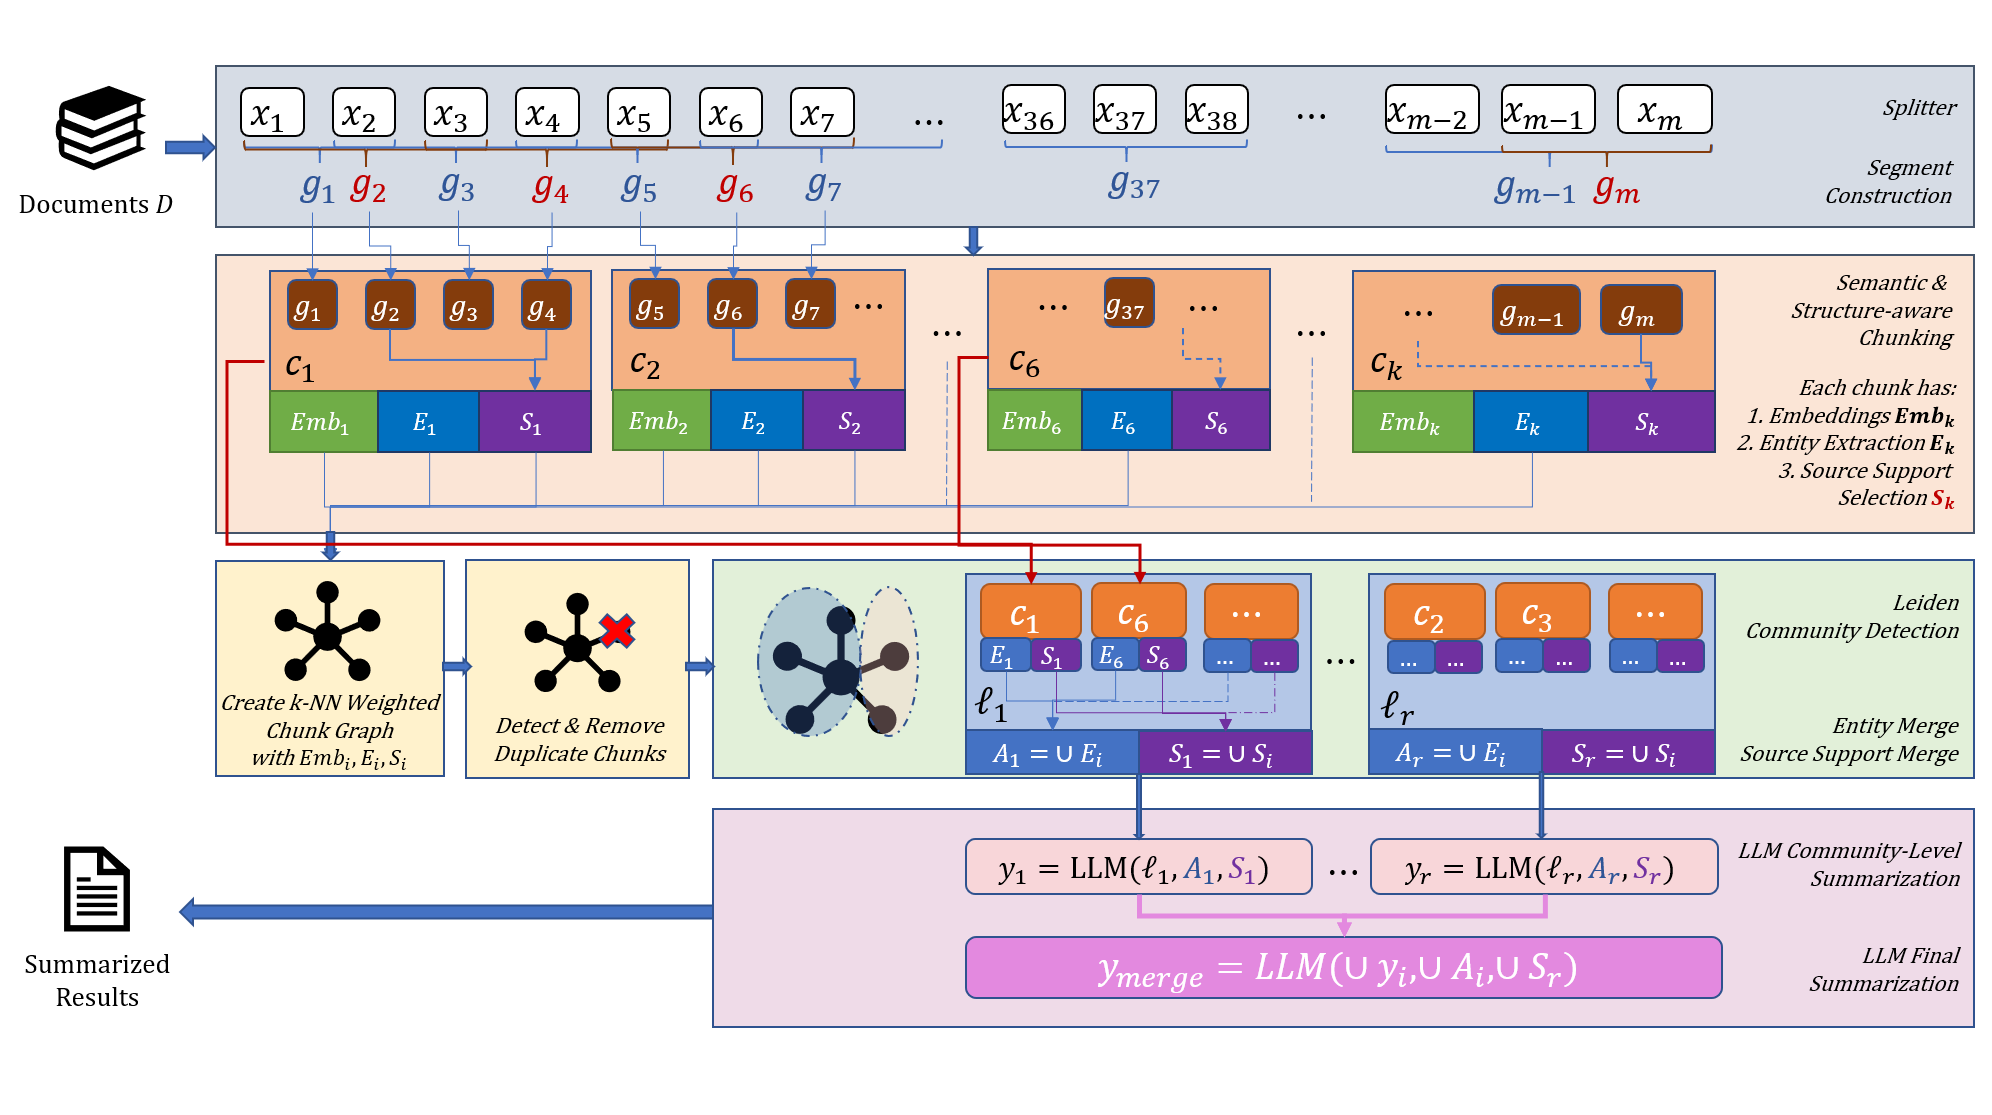
\includegraphics[width=\textwidth]{overview.png}
\caption{Overview of \methodname{}. The framework first constructs source-grounded segments and semantic chunks, then organizes chunks through a weighted graph and Leiden chunk communities. Community-level generation uses ordered source text, selected source support, and factual anchors, while final merging preserves source-only support propagation.}
\label{fig:method-overview}
\end{figure*}


Generated summaries are used for abstraction, while source support remains separately stored and traceable. This separation is the main factuality-oriented constraint of the framework.

\subsection{Segment Construction}

Let $x_i$ denote the $i$-th output of the rule-based sentence-like splitter, based on punctuation marks. The splitter output may be a sentence, headline, clause, fragment, or other sentence-like span. The splitter outputs do not overlap with each other; for document $D$, there are $m$ splitter outputs:
\[
D = [x_1, x_2, \ldots, x_m]
\]

For each index $i \in \{1, \ldots, m\}$, we construct an overlapping segment $g_i$ from up to three consecutive splitter outputs:
\[
g_i = \mathrm{concat}(x_{i-1}, x_i, x_{i+1}).
\]

At document boundaries, only the available neighboring outputs are included, so $g_1=\mathrm{concat}(x_1,x_2)$ and $g_m=\mathrm{concat}(x_{m-1},x_m)$. This produces $m$ overlapping segments $g_1,\ldots,g_m$. Each segment stores its document identifier, source-span identifiers, center index, raw text, and embedding. These segments serve as the atomic support candidates during extraction. Before being passed to the prompting stage, selected overlapping segments are compacted by merging duplicated source spans and restoring them in their original document order.

The three consecutive splitter outputs form a best-effort local context window rather than an assumption that each output is a complete grammatical sentence. This construction helps preserve meaning when punctuation-based splitting separates a short span from the surrounding text on which it depends. For example, in `Does it work? Yes.', the splitter may produce `Does it work?' and `Yes.' as separate outputs, although the meaning of `Yes.' can only be interpreted in relation to the preceding question.


\subsection{Semantic Chunking}

Semantic chunks are larger text units used as graph nodes. BGE-M3 \citep{bge_m3} provides the embeddings used for semantic chunking, segment--chunk similarity, chunk--chunk content similarity, and entity-alias consolidation. We pair it with a semantic chunking procedure implemented through LangChain Experimental SemanticChunker\footnote{\url{https://github.com/langchain-ai/langchain-experimental/blob/main/libs/experimental/langchain_experimental/text_splitter.py}} and preserve paragraph boundaries as structural hints when available. 

Let $c_j$ denote the $j$-th semantic chunk, and let $k$ be the number of chunks, giving $\mathcal{C}=\{c_1,\ldots,c_k\}$. The target chunk size is controlled by lower and upper token budgets $T_{\min}$ and $T_{\max}$. Each chunk stores its text, source segment identifiers, document-relative position, embedding, and canonical phrase set.

\subsection{Entity and Factual Phrase Extraction}

For chunk-level named-entity extraction, \methodname{} uses the tool that is better suited to the input language: Underthesea \citep{underthesea} for Vietnamese and spaCy English NER \citep{honnibal2020spacy} for English. This language-specific routing avoids forcing one library outside its stronger coverage. The NER outputs are augmented with the same rule-based factual phrase layer, which detects dates, percentages, money expressions, and related factual anchors. 

For chunk $c_i$, let $E_i$ denote the set of canonical entities and factual anchors extracted from that chunk. Notice that, we don't perform relation extraction or LLM reasoning between entities: for our graph, co-occurring canonical anchors are sufficient to indicate that two chunks may discuss related facts, while the ordered source text and selected support remain responsible for the actual semantics. Raw phrases are normalized and mapped to chunks.

Named-entity aliases are consolidated with embedding cosine similarity using a merge threshold $\tau_{\mathrm{ent}}$. Numeric, date, and money phrases are not merged by embedding similarity, since doing so could collapse distinct factual values. 

\subsection{Source Support Selection}

A generated summary should not be expected to compress a large semantic chunk without access to the most relevant evidence from the original document, to prevent hallucination. Therefore, for each semantic chunk $c_i$, \methodname{} retains the source segments that contributed to its construction. Let $G_i$ denote this candidate segment set. The support selector chooses a compact subset $S_i \subseteq G_i$ as supporting evidence. This support consists entirely of text copied from the original input rather than a generated intermediate summary; in this sense, it serves as an extractive component of the framework.

Selecting segments based only on their similarity to the chunk may favor highly similar but redundant passages. To obtain a more representative support set, we assign each candidate segment a PACSUM-style centrality score \citep{zheng-lapata-2019-pacsum}, computed from the embedding similarities among the source segments. Segments with higher centrality are more likely to capture information that is broadly important within the chunk.

However, because the segment windows overlap, adjacent candidates can contain repeated text. For instance, $g_1=[x_1,x_2]$, $g_2=[x_1,x_2,x_3]$, and $g_3=[x_2,x_3,x_4]$ share substantial source spans. If $x_1,x_2,x_3,x_4$ are all useful evidence, selecting both $g_1$ and $g_3$ can cover the same information with less redundancy than selecting all three segments. Therefore, a stride parameter $s$ is used to limit the selection of strongly overlapping segments from adjacent windows, thereby reducing near-duplicate evidence. For our testing, we chose $s=2$. 

The selected per-chunk supports $S_i$ are stored separately from generated text and are later combined at the chunk-community level.

\subsection{Sparse Weighted Chunk Graph}

Each semantic chunk is a graph node. Candidate edges are constructed from semantic nearest neighbors and adjacent chunks from the same source document. For candidate chunks $i$ and $j$, the final edge weight is:

\begin{equation}
w_{ij} = \alpha P_{ij} + \beta E_{ij} + \gamma C_{ij},
\end{equation}

where $P_{ij}$ is document-relative positional similarity, $E_{ij}$ is typed TF-IDF cosine similarity between the canonical anchor sets $E_i$ and $E_j$, and $C_{ij}$ is embedding cosine similarity. The graph weights $\alpha$, $\beta$, and $\gamma$ are runtime configuration values that should satisfy:
\begin{equation}
\alpha + \beta + \gamma = 1.
\end{equation}

Positional similarity is only defined within the same document:

\begin{equation}
P_{ij} =
\begin{cases}
\exp(-|p_i - p_j| / \tau), & d_i = d_j, \\
0, & d_i \ne d_j,
\end{cases}
\end{equation}
where $p_i$ is the document-relative chunk position and $d_i$ is the document identifier. We use this term because nearby chunks in the same document are more likely to belong to the same local event, explanation, quotation context, or narrative continuation. The exponential form gives the strongest signal to adjacent chunks and decays smoothly as they move farther apart. For chunks from different documents, relative position is not directly comparable, so the positional term is set to zero and cross-document relatedness is left to entity/factual and content similarity. 

And for $E_{ij}$, each anchor is represented together with its type, such as named entity, date, percentage, or money expression. We then form a sparse TF-IDF vector $\phi(E_i)$ over these typed anchors and compute:

\begin{equation}
E_{ij} = \cos(\phi(E_i), \phi(E_j)).
\end{equation}

This term is high when two chunks share rare, type-compatible anchors, and low when they only share common or unrelated phrases. 


\subsection{Duplicate-Aware Compaction}

Before community detection and prompting, \methodname{} identifies near-duplicate chunks using embedding cosine similarity. Let $\tau_{\mathrm{dup}}$ be the duplicate similarity threshold. Chunks $c_i$ and $c_j$ are assigned to the same duplicate group when their embedding cosine similarity is at least $\tau_{\mathrm{dup}}$, subject to the representative-grouping procedure used by the implementation. During graph construction, edges between chunks in the same duplicate group are downweighted by a duplicate edge factor $\eta_{\mathrm{dup}}$:

\begin{equation}
w'_{ij} = \eta_{\mathrm{dup}} w_{ij}.
\end{equation}

This prevents repeated text from dominating community formation. During prompting, if several chunks from the same duplicate group appear in one community, only the representative is kept in the prompt while the source support trace is preserved. This reduces repeated evidence without deleting the underlying source provenance.


\subsection{Leiden Chunk Communities}

The Leiden algorithm \citep{traag-2019-leiden} is applied to the sparse weighted graph. Let $\ell_t \subseteq \mathcal{C}$ denote the $t$-th detected chunk community, and let $r$ be the number of communities, giving $\mathcal{L}=\{\ell_1,\ldots,\ell_r\}$. The output communities are chunk communities, not assumed linguistic topics. For example, if $\ell_t=\{c_2,c_5,c_6\}$, this only means that the graph links these chunks strongly enough to group them; it does not require that they correspond to a human-labeled topic. Before prompting, chunks inside each $\ell_t$ are sorted back into source order so that the LLM sees the evidence in a coherent reading sequence.

\subsection{Community-Level Extract-Support Generation}

For each chunk community $\ell_t$, the LLM receives three fields. First, the ordered source text is formed by sorting chunks $c_i \in \ell_t$ back into document order and concatenating their text. Second, the compact source-derived support set is the union of the per-chunk supports selected earlier:

\begin{equation}
S_t = \bigcup_{c_i \in \ell_t} S_i.
\end{equation}

Third, the community anchor set is the union of canonical chunk anchors:

\begin{equation}
A_t = \bigcup_{c_i \in \ell_t} E_i.
\end{equation}

The prompt can therefore be viewed as producing a community summary $y_t$ from ordered community text, support $S_t$, and anchors $A_t$:

\begin{equation}
y_t = \mathrm{LLM}(\mathrm{text}(\ell_t), S_t, A_t).
\end{equation}

The anchor set $A_t$ is used as a factual checklist rather than as a source of new relations: the prompt instructs the model to preserve relevant anchors only when they are supported by the text or support evidence. The prompt returns only the summary $y_t$.

If multiple community-level summaries are produced, the system performs a final merge. The merge stage receives generated community summaries $\{y_1,\ldots,y_r\}$ plus source-derived support. Crucially, merge support is not generated text. It is reselected from the union of child support segments:

\begin{equation}
S_{\mathrm{merge}} \subseteq \bigcup_{t=1}^{r} S_t.
\end{equation}

This source-only propagation rule preserves the Extract-Support constraint across hierarchy levels.

\section{Experimental Setup}
\label{sec:experiments}

\subsection{Datasets}

Experiments use 100 samples from each dataset due to time and processing constraints.

\paragraph{VN-MDS.}
VN-MDS\footnote{\url{https://github.com/lupanh/VietnameseMDS}} is used as a Vietnamese multi-document summarization dataset. The current loader reads source documents from local cluster folders using raw article body files and uses the two raw human reference summaries per cluster. Tokenized reference files are excluded from evaluation.

\paragraph{ViMs.}
ViMs \citep{tran2020vims} is a Vietnamese abstractive multi-document summarization dataset. The current loader reads source documents from the `original' folders and uses the two `.gold.txt' summaries as annotator references.

\paragraph{Multi-News.}
Multi-News \citep{fabbri2019multi} is an English multi-document summarization dataset. It is used to test whether the framework transfers when the Vietnamese entity extractor is replaced by an English NER pipeline. 

\subsection{Models and Runtime Configuration}
\methodname{} is a training-free framework that can use different backbone LLMs, although its quality still depends on backbone suitability. BGE-M3 \citep{bge_m3} is used as the embedding model. Gemma4-12B \citep{gemma4_12b} is selected as the LLM model choice in the experiment configuration. LLMs are accessed through an OpenAI-compatible endpoint. All experiments are conducted on one NVIDIA L40S GPU with 48GB VRAM. Used prompt templates are listed in Appendix~\ref{app:prompts}.

The Pure LLM baseline uses the same backbone LLM and summary budgets, but bypasses embeddings, chunking, graph construction, entity extraction, support selection, and hierarchical merging; it directly prompts the LLM with the concatenated source documents. The direct prompt template is listed in Appendix~\ref{app:promptB}. MoA framework \citep{tuan-2026-moa} is included as a competing training-free model and is also equipped with Gemma4-12B through the same OpenAI-compatible endpoint and output budgets.

\begin{table*}[t]
\centering
\small
\setlength{\tabcolsep}{4pt}
\begin{tabular*}{\textwidth}{@{\extracolsep{\fill}}llrrrrrrr@{}}
\toprule
Framework & Dataset & R-1 $\uparrow$ & R-2 $\uparrow$ & R-L $\uparrow$ & Input tok. $\downarrow$ & Output tok. $\downarrow$ & Calls $\downarrow$ & Runtime (s) $\downarrow$ \\
\midrule
\multirow{3}{*}{Pure LLM} & VN-MDS & 68.56 & 45.86 & 38.67 & 2384 & 419 & 1.00 & 6.86 \\
 & ViMs & 73.56 & 47.83 & 40.14 & 4199 & 439 & 1.00 & 7.57 \\
 & Multi-News & 42.64 & 12.07 & 19.73 & 2642 & 313 & 1.00 & 5.31 \\
\addlinespace
\multirow{3}{*}{MoA (\citeyear{tuan-2026-moa})} & VN-MDS & \underline{82.36} & \underline{58.06} & \underline{43.16} & 17119 & 1666 & 8.75 & 28.40 \\
 & ViMs & \underline{83.26} & \underline{60.78} & \textbf{43.05} & 16653 & 1800 & 8.98 & 30.52 \\
 & Multi-News & \underline{43.58} & \textbf{13.35} & \textbf{20.28} & 14787 & 1646 & 9.24 & 27.66 \\
\addlinespace
\multirow{3}{*}{\textbf{\methodname{}(Ours)}} & VN-MDS & \textbf{83.33} & \textbf{59.63} & \textbf{43.80} & 4097 & 373 & 1.51 & 7.95 \\
 & ViMs & \textbf{83.52} & \textbf{60.83} & \underline{42.59} & 7137 & 790 & 2.52 & 16.11 \\
 & Multi-News & \textbf{43.87} & \underline{13.17} & \underline{20.18} & 4942 & 449 & 1.68 & 8.49 \\
\bottomrule
\end{tabular*}
\caption{Main 100-sample results from our runs. R-1, R-2, and R-L denote ROUGE-1, ROUGE-2, and ROUGE-L reported as percentages. Arrows indicate whether higher or lower values are better. For ROUGE columns, bold marks the best value and underline marks the second-best value for each dataset.}
\label{tab:main-results}
\end{table*}

\subsection{Evaluation Metrics}

Summaries are evaluated with ROUGE \citep{lin-2004-rouge}, following the evaluation practice used by many other papers for text summarization tasks. We report ROUGE-1 (R-1) for content overlap, ROUGE-2 (R-2) for fluency and local coherence,
and ROUGE-L (R-L) for structural similarity and overall coherence against reference summaries. Higher scores indicate better summarization quality. For datasets with two human references, each generated summary is scored against both references and a single best reference is selected for reporting all three ROUGE scores.

Efficiency metrics include input token count, output token count, number of LLM calls, and runtime seconds.

\section{Results}
\label{sec:results}

Table~\ref{tab:main-results} reports the main 100-sample results for the three datasets.


The main pattern in Table~\ref{tab:main-results} is that structure helps most when the input is Vietnamese and multi-document. Compared with direct prompting, \methodname{} raises ROUGE-2 by roughly 14 points on VN-MDS and 13 points on ViMs, while also improving ROUGE-L. This suggests that the graph-guided chunk communities and source-support prompts recover evidence that a single long prompt tends to underuse. Multi-News shows a smaller gain, but ROUGE-1 and ROUGE-2 still improve over Pure LLM, which indicates that the pipeline is not tied only to Vietnamese inputs even though its advantage is narrower in English.

The comparison with MoA-MDS shows the intended efficiency trade-off. \methodname{} stays in the same ROUGE range as the competing training-free model, but it reaches that range with far fewer generation resources. On VN-MDS, calls fall from 8.75 to 1.51 and input tokens from 17,119 to 4,097; on ViMs, calls fall from 8.98 to 2.52; on Multi-News, \methodname{} uses about one fifth of the calls and about one third of the input tokens. The result is not simply that \methodname{} gets higher lexical overlap everywhere, but that it preserves competitive quality while shifting much of the work from repeated LLM generation to cheaper source processing and graph organization.

The strongest evidence for \methodname{} is efficiency-adjusted rather than absolute dominance on every metric. The method is especially effective on the Vietnamese datasets, where source wording, redundancy, and entity/factual anchors appear to benefit from chunk-community grouping and source-only support propagation. The weaker Multi-News margin suggests that English generalization is feasible, but dataset-specific tuning of chunk size, graph weights, or support budgets may be needed.

These findings also clarify the role of the graph. The graph is not used as a full knowledge graph for relation reasoning; instead, it organizes chunks before generation and exposes source-grounded support to the LLM. This lighter use of structure is consistent with the efficiency objective: most computation remains in deterministic preprocessing, while the expensive LLM stages are reserved for community-level abstraction and final merging.

\section{Limitations}
\label{sec:limitations}

The current study has several limitations. First, experiments are limited to 100 samples per dataset because of time and processing constraints. Second, the pure LLM baseline may exceed the context window for some samples, depending on the served model configuration. Third, the individual contribution of each component in the proposed framework has not been investigated extensively. Finally, although ROUGE provides a useful measure of lexical overlap, it does not directly evaluate factual consistency or faithfulness to the source documents.

\section{Conclusion}
\label{sec:conclusion}

This paper proposes \methodname{}, a training-free structure-aware, hierarchical, and efficient summarization framework for Vietnamese long-document and multi-document summarization. The method combines overlapping segment evidence, semantic chunks, lightweight entity and factual phrase processing, sparse weighted chunk graphs, Leiden chunk communities, source-only support propagation, and entity-aware prompting after deduplication.

\section*{Code Availability}

The implementation and experimental code are all available at: \url{https://github.com/Legend0fHell/SHESum_Text_Summarization}.

\bibliography{custom}

\clearpage
\onecolumn
\appendix

\section{Selected Hyperparameters}
\label{app:hyperparameters}

Table~\ref{tab:appendix-hyperparams} lists the selected configuration used for the reported \methodname{} runs.

\begin{table*}[t]
\centering
\small
\begin{tabular}{lll}
\toprule
Component & Hyperparameter & Selected value \\
\midrule
Input limit & Samples per dataset & 100 \\
Chunking & Target minimum tokens $T_{\min}$ & 150 \\
Chunking & Target maximum tokens $T_{\max}$ & 1500 \\
Chunking & Semantic breakpoint percentile & 50.0 \\
Chunking & Minimum semantic chunk tokens & 75 \\
Support selection & PACSUM $\beta$ & 0.0 \\
Support selection & PACSUM $\lambda_1$ & 0.0 \\
Support selection & PACSUM $\lambda_2$ & 1.0 \\
Support selection & Stride $s$ & 2 \\
Support selection & Evidence budget & 400 tokens \\
Graph & k-Nearest neighbors & 8 \\
Graph & Position weight $\alpha$ & 0.10 \\
Graph & Entity/factual weight $\beta$ & 0.30 \\
Graph & Content weight $\gamma$ & 0.60 \\
Entity anchors & Entity merge threshold $\tau_{\mathrm{ent}}$ & 0.80 \\
Deduplication & Duplicate similarity threshold $\tau_{\mathrm{dup}}$ & 0.85 \\
Deduplication & Require shared phrase & No \\
Deduplication & Duplicate edge factor $\eta_{\mathrm{dup}}$ & 0.35 \\
Deduplication & Community prompt deduplication & Enabled \\
LLM & Model & Gemma4-12B \\
LLM & Temperature & 0.6 \\
LLM & Maximum summary length & 250 words \\
LLM & Maximum output tokens & 400 tokens \\
\bottomrule
\end{tabular}
\caption{Selected hyperparameters for the reported \methodname{} runs.}
\label{tab:appendix-hyperparams}
\end{table*}

\section{Prompt Templates}
\label{app:prompts}

The following templates are the prompt templates used by the implementation. Runtime placeholders such as \texttt{\{language\_name\}}, \texttt{\{source\_text\}}, and \texttt{\{entities\}} are filled for each sample.

\subsection{Community-Level Extract-Support Prompt}
\label{app:promptA1}

\begingroup
\tiny
\begin{verbatim}
[Instruction]
You are a multilingual, fact-grounded community summarization agent.
Write in {language_name}. Your role is to summarize one chunk community
using ordered source text and selected source support.

[Objective]
Given:
1. Ordered source text from one chunk community.
2. Source support selected from original source segments.
3. Canonical entities and factual anchors extracted from the community
   chunks after deduplication.

Produce a coherent community-level summary that:
- captures the central event, actors, actions, causes, consequences, and
  important context;
- preserves salient entities, numbers, dates, locations, and factual phrases;
- acknowledges disagreement, uncertainty, or contrast when the sources support it;
- remains strictly grounded in the provided input and does not add external knowledge.

[Dataset guidance]
{dataset_guidance}

[Length constraint]
{length_constraint}

[Process]
1. Identify Core Content
 - Determine the main event or situation, the central actors, and the most
   important actions or outcomes.
 - Use the ordered source text for coverage and narrative flow.
2. Verify Against Support
  - Prefer claims grounded in the selected source support when details are ambiguous.
  - Keep concrete facts only when supported by the source text or source support.
3. Use Entity and Factual Anchors
  - Treat the entity list as a checklist of names, organizations, locations,
    dates, numbers, money amounts, and other factual anchors that may be important.
  - Include an entity or factual anchor only when it is relevant to the main event
    and supported by the source text or source support.
  - Do not invent relationships between listed entities; the list is not a
    knowledge graph and does not by itself prove a claim.
4. Compose
  - Write clear, neutral prose in inverted-pyramid style: most important
    information first, context after.
  - Merge repeated information once.
  - Do not mention "source text", "source support", "entity list", "chunk",
    "community", "segment", "prompt", or the summarization process.

[Input]
Source text:
---
{source_text}
---

Source support:
---
{source_support}
---

Canonical entities and factual anchors:
---
{entities}
---

[Output]
Return ONLY the final summary as plain text. Do not include labels, headings,
bullet points, metadata, JSON, or analysis.
\end{verbatim}
\endgroup

\subsection{Final Merge Prompt}
\label{app:promptA2}

\begingroup
\tiny
\begin{verbatim}
[Instruction]
You are a multilingual, metadata-aware summary synthesizer. Write in {language_name}.
Your task is to fuse multiple community-level summaries into one coherent final
summary while using source-derived support only for factual verification.

[Objective]
Given:
1. Community-level summaries generated from chunk communities.
2. Source-derived support inherited from the original source segments.
3. Canonical entities and factual anchors extracted from deduplicated community chunks.

Produce a final integrated summary that:
- preserves the main information from all important community summaries;
- emphasizes globally central facts and relationships;
- removes redundancy across communities;
- keeps numerical, temporal, and entity-specific details only when supported;
- explicitly preserves major disagreements, caveats, or uncertainty when supported.

[Dataset guidance]
{dataset_guidance}

[Length constraint]
{length_constraint}

[Process]
1. Rank and Integrate
 - Identify which community summaries contain the global lead, supporting context,
   consequences, and caveats.
 - Merge repeated claims once and preserve complementary details.
2. Verify and Resolve
  - Use source-derived support to check factual accuracy.
  - If summaries conflict, state the contrast only when the source-derived support
    justifies it; otherwise use cautious wording.
3. Use Entity and Factual Anchors
  - Use the entity list as a factual checklist while merging, especially for names,
    organizations, locations, dates, numbers, and monetary facts.
  - Preserve anchors that are globally important and supported; omit anchors that
    are peripheral, repeated, or unsupported by the summaries/support.
  - Do not infer new relationships solely because entities appear together in the list.
4. Compose Final Summary
  - Use inverted-pyramid structure: lead first, context and consequences after.
  - Do not reference "community summaries", "source support", "entity list",
    "metadata", "chunks", "segments", or the summarization process.

[Input]
Community summaries:
---
{topic_summaries}
---

Source-derived support:
---
{source_support}
---

Canonical entities and factual anchors:
---
{entities}
---

[Output]
Return ONLY one final summary as plain text. Do not include labels, headings,
bullet points, metadata, JSON, or analysis.
\end{verbatim}
\endgroup

\subsection{Direct LLM Reference Prompt}
\label{app:promptB}

\begingroup
\tiny
\begin{verbatim}
[Instruction]
You are a multilingual, fact-grounded multi-document summarization model. Write in
{language_name}. Do not add information that is not present in the source documents.

[Objective]
Given a collection of related source documents, produce a concise, neutral summary that:
- captures the main point, key entities, events, relationships, numbers, dates,
  and causal links;
- merges repeated information across documents;
- preserves critical nuance, disagreement, uncertainty, or contrast when present;
- avoids opinion, hype, speculation, and hallucination.

[Dataset guidance]
{dataset_guidance}

[Length constraint]
{length_constraint}

[Process]
1. Multi-Document Scan
 - Identify recurring themes, central actors, core events, major claims, and
   salient factual details.
2. De-duplicate and Reconcile
 - Merge repeated details.
 - If conflicting claims exist, briefly note the disagreement without resolving it
   beyond what the documents state.
3. Compose
 - Write clear, neutral prose in inverted-pyramid style.
 - Do not mention "source documents", "prompt", or the summarization process.

[Input]
Source documents:
---
{source_text}
---

[Output]
Return ONLY the final summary as plain text. Do not include labels, headings,
bullet points, metadata, JSON, or analysis.
\end{verbatim}
\endgroup

\end{document}
